\documentclass[11pt,a4paper]{article}
\usepackage[utf8]{inputenc}
\usepackage[T1]{fontenc}
\usepackage{amsfonts}
\usepackage{amssymb}
\usepackage{mdframed}
\usepackage{tikz}
\usepackage{tkz-tab}
\usepackage{xcolor}
\usepackage{fancyhdr}
\usepackage{lastpage}
\usepackage[fleqn]{amsmath}
\usepackage{siunitx}
\usepackage{pgfplots}
\pgfplotsset{compat = newest}
\setlength{\mathindent}{0pt}

% Spécifications du document
\newcommand{\doctitre}{Les suites} % Ex: Le second degré
\newcommand{\docniveau}{$1^{\text{re}}$ Spécialité mathématiques} % Ex: $1e^{\text{re}}$ Spécialité mathématiques
\newcommand{\doctheme}{Algèbre } % Ex: Algèbre
\newcommand{\doctype}{Cours} % Ex: Démonstrations
\newcommand{\docshorttype}{Cours} % Ex : Démo

% Couleurs pour les graphiques
\definecolor{dark_green}{HTML}{008000}

% Paramètres du document
\RequirePackage{geometry}
\geometry{tmargin=1cm,bmargin=1.9cm,lmargin=1.9cm,rmargin=1.9cm}
\renewcommand{\familydefault}{\sfdefault}
\setlength{\parindent}{0pt}
\title{\doctitre}
\author{\docniveau \\ \doctheme - \doctype}
\date{}
\fancypagestyle{custom}{
  \fancyhf{}
  \renewcommand{\headrulewidth}{0pt}
  \lfoot{\doctheme - \docshorttype}
  \cfoot{\doctitre} % Change \titre to \doctitre
  \rfoot{\thepage/\pageref{LastPage}}
}

% Styles pour les mdframed
\mdfdefinestyle{definitionStyle}{
    leftline=true,
    rightline=false,
    topline=false,
    bottomline=false,
    linewidth=2pt,
    linecolor=black,
    innertopmargin=0pt,
    innerbottommargin=0pt,
    innerrightmargin=0pt,
    innerleftmargin=5pt,
}

\mdfdefinestyle{proprieteStyle}{
    linewidth=1pt,
    linecolor=black,
    innertopmargin=5pt,
    innerbottommargin=5pt,
    innerrightmargin=5pt,
    innerleftmargin=5pt,
}

% ----- DEBUT DU DOCUMENT -----
\begin{document}

% Style et numérotation
\maketitle
\pagestyle{custom}
\thispagestyle{custom}

% Sections et sous-sections
\section*{I. Généralités}
\subsection*{1. Introduction}

\begin{mdframed}[style=definitionStyle]
  \textbf{Définitions :} ~\\
  Une suite numérique $u$ est une fonction $u:n \mapsto u(n)$ définie pour tout entier naturel $n$
  (ou tout entier naturel $n \geq k$, $k$ étant un entier naturel).
  \vspace{-4pt}
  \begin{itemize}
    \item  $u(n)$ ou $u_n$ s'appelle le terme de rang $n$ (ou le terme général de la suite).
    \item  $u$ désigne la suite elle-même, elle peut être noté aussi $(u_n)$.
    \item  $n$ est l'indice (ou le rang).
    \item  $u_{n-1}$ est le terme précédant $u_n$.
    \item  $u_{n+1}$ est le terme suivant $u_n$.
    \item  $u_0$ (ou parfois $u_1$) est le terme initial (ou le premier terme).
  \end{itemize}

\end{mdframed}

\subsection*{2. Différents modes de génération d'une suite}

\begin{mdframed}[style=definitionStyle]
  \textbf{Définition :} ~\\
  Une suite est définie de façon explicite lorsqu'on peut calculer n'importe quel terme de la suite directement en fonction de $n$.
\end{mdframed}

\textbf{Exemple :} ~\\
Soit la suite $u$ définie par $u_n=12+2n$ pour tout entier naturel. \\
On calcule ses premiers termes :
\vspace{-8pt}
\begin{equation*}
  \begin{split}
    &u_0=12+2\times0=12\\
    &u_1=12+2\times1=14\\
    &u_2=12+2\times2=16
  \end{split}
  \qquad\qquad
  \begin{split}
    &u_3=12+2\times3=18\\
    &u_4=12+2\times4=20\\
    &u_5=12+2\times5=22
  \end{split}
\end{equation*}


\begin{mdframed}[style=definitionStyle]
  \textbf{Définition :} ~\\
  Lorsqu'une suite est définie par la donnée de son premier terme et d'une relation qui permet de calculer chaque
  terme en fonction du terme précédent, on dit que la suite est définie par récurrence.
  On donne l'expression de $u_{n+1}$ en fonction de $u_n$. \\ Cette relation s'appelle relation (ou formule) de récurrence.
\end{mdframed}

\textbf{Exemple :} ~\\
Soit $F$ la suite définie par
$\left\{
  \begin{array}{l}
    F_0=0 \\
    F_1=1 \\
    F_{n+1}=F_{n-1}+F_{n-2}
  \end{array}
  \right.$ pour tout $n\geq2$.\\

Cette suite s'appelle la suite de Fibonacci. Elle est définie par une relation de récurrence d'ordre 2, c'est à dire
que chaque terme de la suite est la somme des deux termes qui le précèdent.
\begin{equation*}
  \begin{split}
    &F_2=1+0=1\\
    &F_3=1+1=2
  \end{split}
  \qquad\qquad\qquad
  \begin{split}
    &F_4=2+1=3\\
    &F_5=3+2=5
  \end{split}
  \qquad\qquad\qquad
  \begin{split}
    &F_6=5+3=8\\
    &F_7=8+5=13
  \end{split}
  \qquad\qquad\qquad
  \begin{split}
    &F_8=13+8=21\\
    &F_9=21+13=34
  \end{split}
\end{equation*}

\newpage

\subsection*{3. Représentation graphique d'un suite}


Une suite $u$ peut être représentée :
\vspace{-4pt}
\begin{itemize}
  \item en plaçant les points de coordonnées $(n, u_n)$ dans un repère (on appelle cet ensemble nuage de points).
  \item en plaçant les réels $u_0$, $u_1$, $u_2\dots$ sur une droite graduée.
\end{itemize}


\textbf{Exemple :} ~\\
On représente la suite $u$ définie pour tout entier naturel $n$ par $u_n=n^2-4n+2$.\\
On a  $u_0=2$, $u_1=-1$, $u_2=-2$, $u_3=-1$ et $u_4=2$. \\

\begin{minipage}{0.5\textwidth}
  \centering
  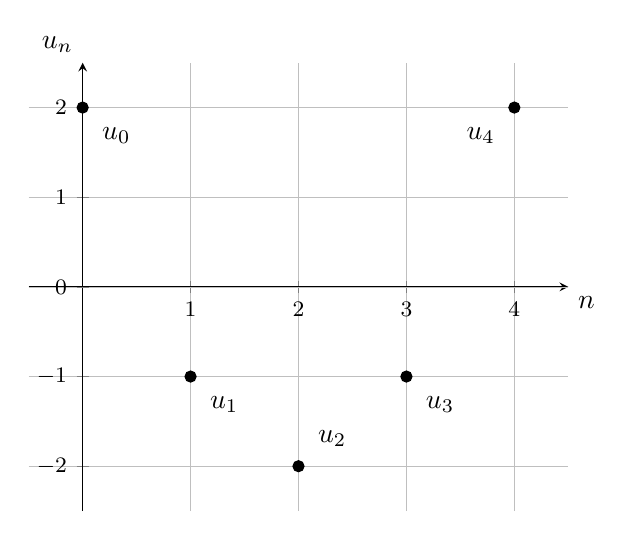
\begin{tikzpicture}
    \begin{axis}[
        axis lines=middle,
        xlabel={$n$},
        ylabel={$u_n$},
        xmin=-0.5,
        xmax=4.5,
        ymin=-2.5, ymax=2.5,
        xtick={0,1,2,3,4},
        ytick={-2,-1,0,1,2},
        xlabel style={below right},
        ylabel style={above left},
        tick label style={font=\footnotesize},
        grid=both,
        major grid style={line width=.2pt,draw=gray!50},
        minor tick num=0,
        extra y ticks={0},
        extra y tick style={grid=major}]
      \addplot[mark=, mark size=2, only marks] coordinates {(0,2)};
      \node[label={below right:$u_0$}] at (axis cs:0,2) {};
      \addplot[mark=, mark size=2, only marks] coordinates {(1,-1)};
      \node[label={below right:$u_1$}] at (axis cs:1,-1) {};
      \addplot[mark=, mark size=2, only marks] coordinates {(2,-2)};
      \node[label={above right:$u_2$}] at (axis cs:2,-2) {};
      \addplot[mark=, mark size=2, only marks] coordinates {(3,-1)};
      \node[label={below right:$u_3$}] at (axis cs:3,-1) {};
      \addplot[mark=*, mark size=2, only marks] coordinates {(4,2)};
      \node[label={below left:$u_4$}] at (axis cs:4,2) {};
    \end{axis}
  \end{tikzpicture}
\end{minipage}%
\begin{minipage}{0.5\textwidth}
  \centering
  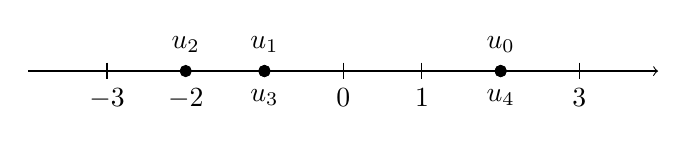
\begin{tikzpicture}
    \draw[->] (-4,0) -- (4,0);
    \foreach \x in {-3,0,1,3}
    \draw (\x cm,3pt) -- (\x cm,-3pt);
    \foreach \x/\label in {-3/-3,-2/-2,0/0,1/1,3/3}
    \node[anchor=north] at (\x cm,-3pt) {$\label$};
    \draw[fill=black] (2,0) circle (2pt) node[above=3pt] {$u_0$};
    \draw[fill=black] (-1,0) circle (2pt) node[above=3pt] {$u_1$};
    \draw[fill=black] (-2,0) circle (2pt) node[above=3pt] {$u_2$};
    \draw[fill=black] (-1,0) circle (2pt) node[below=3pt] {$u_3$};
    \draw[fill=black] (2,0) circle (2pt) node[below=3pt] {$u_4$};
  \end{tikzpicture}
\end{minipage}

\subsection*{4. Sens de variation d'une suite}

\begin{mdframed}[style=definitionStyle]
    \textbf{Définition :} ~\\
    Soit une suite $u$ définie sur $\mathbb{N}$.
    \vspace{-4pt}
    \begin{itemize}
      \item Dire que $u$ est strictement croissante signifie que pour tout $n\in\mathbb{N}$, on a $u_{n+1}>u_n$.
      \item Dire que $u$ est strictement décroissante signifie que pour tout $n\in\mathbb{N}$, on a $u_{n+1}<u_n$.
      \item Dire que $u$ est constante signifie que pour tout $n\in\mathbb{N}$, on a $u_{n+1}=u_n$.
    \end{itemize}

\end{mdframed}

\textbf{Remarques :}
\begin{itemize}
  \item Lorsqu'une suite est croissante ou décroissantes, on dit qu'elle est monotone. 
  \item Pour étudier le sens de variation d'une suite, on peut :
  \vspace{-4pt}
  \begin{enumerate}
    \item calculer la différence $u_{n+1}-u_n$ et étudier son signe.
    \item pour une suite positive, calculer le quotient $\displaystyle\frac{u_{n+1}}{u_n}$ et étudier sa position par rapport à $1$.
    \item pour une suite définie de façon explicite par $u_n=f(n)$, utiliser le sens de variation de $f$. \\
  \end{enumerate}
\end{itemize}
\textbf{Exemple :} ~\\
Soit $u$ définie par $u_n=\frac{1}{3^n}$ pour tout $n\in\mathbb{N}$.

Pour tout $n\in\mathbb{N}$, $u_n>0$ donc on utilise la deuxième méthode.

On calcule $\displaystyle\frac{u_{n+1}}{u_n}=\frac{\frac{1}{3^{n+1}}}{\frac{1}{3^n}}=\frac{1}{3^{n+1}}\times\frac{3^n}{1}=\frac{3^n}{3^{n+1}}=\underbrace{\frac{\overbrace{3\times3\times...\times3}^{\text{$n$ fois}}\color{dark_green}\times1}{3\times3\times...\times3\times3}}_{\text{$n+1$ fois}}=\frac{1}{3}$

\newpage

\section*{II. Suites arithmétiques et géométriques}
\subsection*{1. Suites arithmétiques}
\begin{mdframed}[style=definitionStyle]
  \textbf{Définition :} ~\\
  On dit que la suite $u$ est arithmétique si, à partir de son premier terme, chaque terme est obtenu en ajoutant au
  précédent un même nombre appelé raison. \\
  Pour tout $n\in\mathbb{N}$, $u_{n+1}=u_n+r$
\end{mdframed}

\textbf{Remarque :} Une suite est arithmétique si $u_{n+1}-u_n=r$ pour tout $n\in\mathbb{N}$.

\begin{mdframed}[style=proprieteStyle]
    \textbf{Propriété \emph{(formule explicite)}:} ~\\
    Soit $u$ une suite arithmétique de raison $r$. \\
    Alors, pour tout $n\in\mathbb{N}$, $u_n=u_0+nr$. \\
    Plus généralement, pour tout entier $n$ et $p$, $u_n=u_p+(n-p)r$
\end{mdframed}

\begin{mdframed}[style=proprieteStyle]
    \textbf{Théorème \emph{(sens de variation)} :} ~\\
    Soit $u$ une suite arithmétique de raison $r$.
    \begin{itemize}
      \item Si $r>0$, la suite $u$ est strictement croissante.
      \item Si $r<0$, la suite $u$ est strictement décroissante.
      \item Si $r=0$, la suite $u$ est constante.
    \end{itemize}
\end{mdframed}

\begin{mdframed}[style=proprieteStyle]
    \textbf{Propriété \emph{(représentation graphique)} :} ~\\
    La représentation graphique d'une suite arithmétique est un nuage de points situé sur une droite d'équation $y=u_0+xr$.
\end{mdframed}

\textbf{Exemple :} ~\\
On représente la suite arithmétique de premier terme $u_0=1$ et de raison $r=2$ :\\ \\
\begin{minipage}[t]{0.4\textwidth}
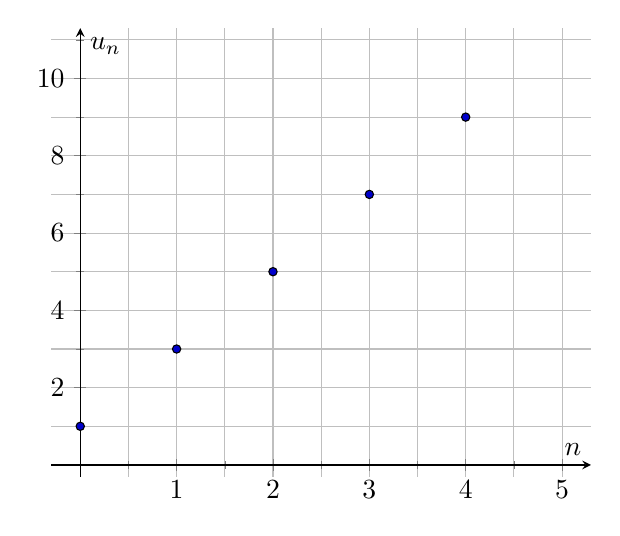
\begin{tikzpicture}
\begin{axis}[
  xlabel={$n$},
  ylabel={$u_n$},
  axis lines=middle,
  grid=both,
  minor tick num=1,
  enlargelimits={abs=0.3},
  ymin=0,
  ymax=11,
  xmin=0,
  xmax=5
]
\addplot+[ycomb, black, mark=*, mark size=1.5pt, only marks, samples at={0,1,2,3,4}] {1+2*x};
\end{axis}
\end{tikzpicture}
\end{minipage}
\hfill
\begin{minipage}[t]{0.55\textwidth}
\vspace{-100pt}
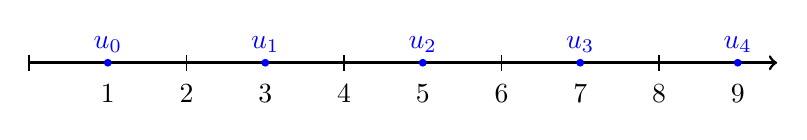
\begin{tikzpicture}
  % Dessinez la droite graduée
  \draw[line width=1pt, ->] (0,0) -- (9.5,0);
  
  % Ajoutez les graduations
  \foreach \x in {0, 2, 4, 6, 8} {
    \draw[line width=0.6pt] (\x, 0.1) -- (\x, -0.1);
  }
  
  % Ajoutez les étiquettes de graduation
  \foreach \x/\n in {1/1,2/2,3/3,4/4,5/5,6/6,7/7,8/8,9/9} {
    \node[below] at (\x, -0.15) {$\n$};
  }
  
  % Dessinez les points de la suite
  \foreach \x in {1,3,5,7,9} {
    \node[blue, fill, circle, inner sep=1pt] at (\x, 0) {};
  }
  
  % Ajoutez les étiquettes des points
  \foreach \x/\n in {1/u_0,3/u_1,5/u_2,7/u_3,9/u_4} {
    \node[blue, above] at (\x, 0) {$\n$};
  }
\end{tikzpicture}
\end{minipage}

\begin{mdframed}[style=proprieteStyle]
    \textbf{Théorème \emph{(calculs de sommes de termes consécutifs)} :} ~\\
    Soit $n$ un entier naturel non nul. \\
    Alors la somme des $n$ premiers termes non nuls est $\displaystyle 1+2+3+...+n=\frac{n(n+1)}{2}$.
\end{mdframed}

\textbf{Exemple :}
\vspace*{-8px}
\begin{align*}
  \text{On calcule }S&=1+2+3+\dots+1\text{ }000 \\
  &=\frac{1\text{ }000(1\text{ }000+1)}{2} \\
  &=500\text{ }500
\end{align*}

\newpage

\subsection*{2. Suites géométriques}

\begin{mdframed}[style=definitionStyle]
  \textbf{Définition :} ~\\
  On dit que la suite $u$ est géométrique si, à partir de son premier terme, chaque terme est obtenu en multipliant le
  précédent par un même nombre appelé raison. \\
  Pour tout $n\in\mathbb{N}$, $u_{n+1}=u_n\times q$
\end{mdframed}

\textbf{Remarque :} Une suite est géométrique si $\frac{u_{n+1}}{u_n}=q$ pour tout $n\in\mathbb{N}$.

\begin{mdframed}[style=proprieteStyle]
    \textbf{Propriété \emph{(formule explicite)} :} ~\\
    Soit $u$ une suite géométrique de raison $q$. \\
    Alors, pour tout $n\in\mathbb{N}$, $u_n=u_0\times q^n$. \\
    Plus généralement, pour tout entier $n$ et $p$, $u_n=u_p\times q^{n-p}$
\end{mdframed}

\begin{mdframed}[style=proprieteStyle]
    \textbf{Théorème \emph{(sens de variation)} :} ~\\
    Soit $u$ une suite géométrique de raison $q$ et de premier terme $u_0$ strictement positif.
    \begin{itemize}
      \item Si $q>1$, la suite $u$ est strictement croissante.
      \item Si $q=1$, la suite $u$ est constante, égal à $u_0$.
      \item Si $0<q<1$, la suite $u$ est strictement décroissante.
      \item Si $q=0$, la suite $u$ est constante égale à $0$, à partir du rang $1$.
      \item Si $q<0$, la suite $u$ n'est ni croissante ni décroissante.
    \end{itemize}
\end{mdframed}

\begin{mdframed}[style=proprieteStyle]
    \textbf{Propriété \emph{(représentation graphique)} :} ~\\
    La représentation graphique d'une suite géométrique est un nuage de points situé sur la courbe d'une fonction exponentielle.
\end{mdframed}

\textbf{Exemple :} ~\\
On représente la suite géométrique de premier terme $u_0=1$ et de raison $q=1,5$ :\\ \\
\begin{minipage}[t]{0.4\textwidth}
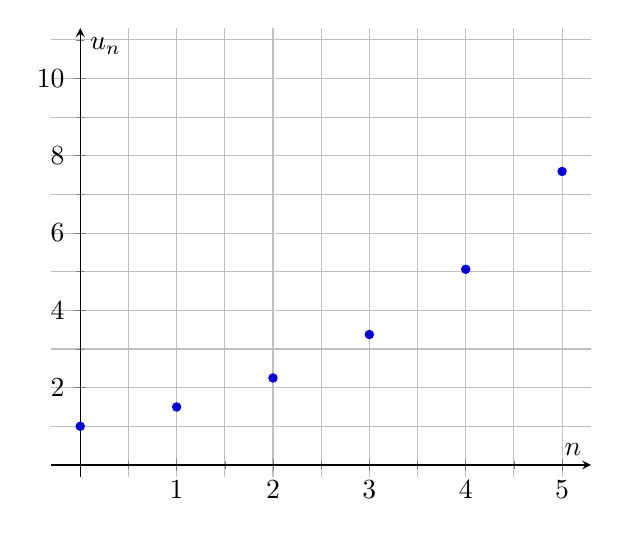
\begin{tikzpicture}
\begin{axis}[
  xlabel={$n$},
  ylabel={$u_n$},
  axis lines=middle,
  grid=both,
  minor tick num=1,
  enlargelimits={abs=0.3},
  ymin=0,
  ymax=11,
  xmin=0,
  xmax=5
]
\addplot+[ycomb, blue, mark=*, mark size=1.5pt, only marks, samples at={0,1,2,3,4, 5}] {1*1.5^x};
\end{axis}
\end{tikzpicture}
\end{minipage}
\hfill
\begin{minipage}[t]{0.55\textwidth}
\vspace{-100pt}
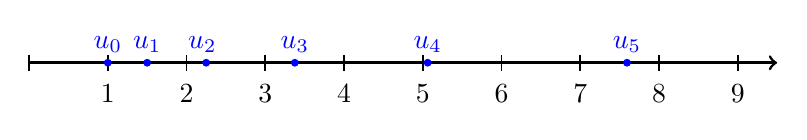
\begin{tikzpicture}
  % Dessinez la droite graduée
  \draw[line width=1pt, ->] (0,0) -- (9.5,0);
  
  % Ajoutez les graduations
  \foreach \x in {0,1,...,9} {
    \draw[line width=0.6pt] (\x, 0.1) -- (\x, -0.1);
  }
  
  % Ajoutez les étiquettes de graduation
  \foreach \x/\n in {1/1,2/2,3/3,4/4,5/5,6/6,7/7,8/8,9/9} {
    \node[below] at (\x, -0.15) {$\n$};
  }
  
  % Dessinez les points de la suite
  \foreach \x in {1,1.5, 2.25, 3.375, 5.0625, 7.59375} {
    \node[fill, blue, circle, inner sep=1pt] at (\x, 0) {};
  }
  
  % Ajoutez les étiquettes des points
  \foreach \x/\n in {1/u_0, 1.5/u_1, 2.2/u_2, 3.375/u_3, 5.0625/u_4, 7.59375/u_5} {
    \node[blue, above] at (\x, 0) {$\n$};
  }
\end{tikzpicture}
\end{minipage}

\begin{mdframed}[style=proprieteStyle]
    \textbf{Théorème \emph{(calculs de sommes de termes consécutifs) :}} ~\\
    Soit $n$ un entier naturel non nul et $q$ un réel différent de $1$. \\
    Alors $\displaystyle 1+q+q^2+...+q^n=\frac{1-q^{n+1}}{1-q}$.
\end{mdframed}

\textbf{Exemple :}
\vspace*{-8px}
\begin{align*}
  \text{On calcule }S&=1+2+2^2+2^3+\dots+2^{10} \\
  &=\frac{1-2^{11}}{1-2} \\
  &=2\text{ }047
\end{align*}

\newpage

\section*{III. Suites minorées et majorées}

\begin{mdframed}[style=definitionStyle]
    \textbf{Définition :} ~\\
    Soit $u$ une suite.
    \vspace*{-4pt}
    \begin{itemize}
      \item On dit que $u$ est minorée s'il existe un réel $m$ tel que pour tout $n\in\mathbb{N}, u_n\geq m$.
      On dit que $m$ est un minorante de la suite.
      \item On dit que $u$ est majorée s'il existe un réel $M$ tel que pour tout $n\in\mathbb{N}, u_n\leq m$.
      On dit que $M$ est un majorant de la suite.
    \end{itemize} 
\end{mdframed}

\textbf{Remarques :}
\begin{itemize}
  \item Une suite croissante est nécesairement minorée par son terme initial : $\forall n\in\mathbb{N}, u_n\geq u_0$.
  \item Une suite décroissante est nécesairement majorée par son terme initial : $\forall n\in\mathbb{N}, u_n\leq u_0$.
\end{itemize} 

\textbf{Exemple :}
\begin{itemize}
  \item On pose $\forall n\in\mathbb{N}^*, u_n=\frac{-1}{n}$. \\
  La suite $(u)$ est strictement croissante car $\forall n\in\mathbb{N}^*, n<n+1 \Rightarrow \frac{1}{n}>\frac{1}{n+1}\Rightarrow\frac{-1}{n}<\frac{-1}{n+1}$. \\
  Donc $(u)$ est majorée par $0$ : $\forall n\in\mathbb{N}^*, \frac{-1}{n}\leq0$.
  \item On pose 
  $u_n=\left\{
  \begin{array}{l}
    -n \text{ si $n$ pair} \\
    n \text{ si $n$ impair}
  \end{array}
  \right.$ pour tout $n\in\mathbb{N}$. La suite$(u)$ n'est ni minorée ni majorée.
\end{itemize}


\section*{IV. Propositions héréditaires et démonstrations par récurrence}

\begin{mdframed}[style=definitionStyle]
    \textbf{Définition :} ~\\
    Soit $P(n)$ un prédicat de $n$. \\
    On dit que $P$ est héréditaires si la proposition « $\forall n\in\mathbb{N}, \text{ } P(n)\Rightarrow P(n+1)$ » est vérifiée.	
\end{mdframed}

\textbf{Exemple :}
\begin{itemize}
  \item Soit $P(n)$ : « $n^2>10$ » pour tout $n\in\mathbb{N}$. $P(0)$, $P(1)$, $P(2)$ et $P(3)$ sont fausses. \\
  Ensuite, $P(4)$, $P(5)$, etc sont vraies et ceci pour tout $n\geq4$ (preuve : $f(x)=x^2$ est croissante sur $[0;+\infty[$ et $f(4)=16$).\\
  Donc $P$ est héréditaires.	
  \item Soit $P(n)$ : « $\frac{6}{n+1}>1,1$ » pour tout $n\in\mathbb{N}$. $P(0)$, $P(1)$, $P(2)$ $P(3)$ et $P(4)$ sont vraies.\\
  Ensuite, $P(5)$, $P(6)$, etc sont fausses et ceci pour tout $n\geq5$ (preuve : si $n\geq5$, alors $n+1\geq6$ donc $\frac{6}{n+1}\leq\frac{6}{6}=1$).\\
  Donc $P$ n'est pas héréditaires car $P(4)$ est vraie mais $P(5)$ est fausse ce qui contredit « $P(n)\Rightarrow P(n+1)$ ».
\end{itemize}

\begin{mdframed}[style=proprieteStyle]
    \textbf{Théorème :} ~\\
    Soit $P(n)$ un prédicat de $n$. On suppose que $P(n)$ est héréditaire.\\
    Deux cas sont alors possibles :
    \vspace{-4pt}
    \begin{itemize}
      \item $P(n)$ est fausse pour tout $n\in\mathbb{N}$.
      \item il existe un entier $n_0$ tel que $P(n)$ soit vraie pour tout entier $n\geq n_0$.
    \end{itemize}
\end{mdframed}

\textbf{Remarque :} Faire une « démonstration par récurrence » consiste à prouver qu'une proposition $P$ est héréditaire 
et trouver un entier $n_0$ pour lequelle $P(n_0)$ est vraie.\\
Le principe de récurrence permet alors de conclure que pour tout entier naturel $n\geq n_0$, $P(n)$ est vraie.	

\newpage

\textbf{Exemple d'une démonstration par récurrence :} ~\\

Soit la suite 
$\left\{
  \begin{array}{l}
    u_0 = 3 \\
    u_n+1 = \frac{u_n}{2} + 1
  \end{array}
  \right. \text{.}$\\
  
  Nommons $P(n)$ : « $u_n\leq3$ ».
  \begin{itemize}
    \item \underline{Initialisation :}\\
    $P(0)$ est vraie car $u_0=3$.
    \item \underline{Hérédité :}\\
    Montrons que $P$ est héréditaire.\\
    Soit $n$ un entier naturel. Supposons $P(n)$ :
    \vspace{-4pt}
  \begin{flalign*}
    &\text{On a } u_n \leq 3 \\
    &\text{donc } \frac{u_n}{2} \leq 1,5 \\
    &\text{donc } \frac{u_n}{2}+1 \leq 2,5 \\
    &\text{donc } \frac{u_n}{2}+1 \leq 2,5 \leq 3 \\
    &\text{donc } u_{n+1} \leq 3 \text{ donc $P(n+1)$}
  \end{flalign*}
  \item \underline{Conclusion :}\\
  Par principe de récurrence, comme $P$ est héréditaire et vraie au rang $0$, on déduit que pour tout $n\geq0$, $P(n)$ est vraie.\\
  Autrement dit, pour tout $n\geq0$, $u_n\leq3$. 
  \end{itemize}
\vspace{4pt}
\textbf{Remarque :} En math, supposer $\not=$ admettre. Lorsqu'on suppose, on attribut temporairement la valeur de vérité « vrai »
à une proposition (on suppose souvent lors de démonstrations) tandis que lorsqu'on admet, on suppose de manière définitive 
(ex : on admet des théorèmes lorsqu'ils sont trop complexes pour être démontrés).

\section*{V. Comportement d'une suite à l'infini}

S'intéresser à la limite d'une suite, c'est étudier le comportement des termes $u_n$ quand on donne des valeurs à $n$ aussi grandes que l'on veut, ce qui se dit aussi : « quand $n$ tend vers l'infini ».  \\

On s'intéresse aux suite $\color{red}u$, $\color{blue}v$, $\color{dark_green}w$, $\color{orange}x$ et $t$ définies pour tout entier naturel $n$ par : 
$$
\color{red}u_n=\frac{1}{n} \quad\quad\quad \color{blue}v_n=\frac{4n-5}{2n+3} \quad\quad\quad \color{dark_green}w_n = n^2 \quad\quad\quad \color{orange}x_n=16-2n^2 \quad\quad\quad \color{black}t_n= (-1)^n
$$

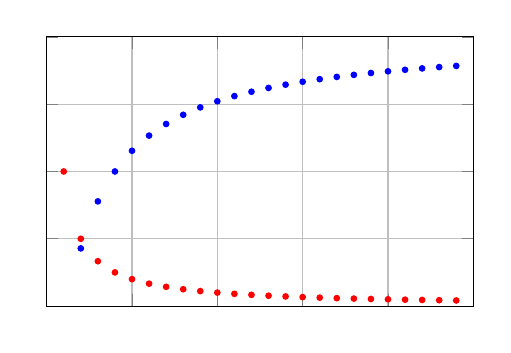
\begin{tikzpicture}
  \begin{axis}[
      xmin=0, xmax=25,
      ymin=0, ymax=2,
      width=7cm, height=5cm,
      grid=major,
      xticklabels={},  % Remove x-axis tick labels
      yticklabels={}
  ]
    
  \foreach \x in {1,2,...,24} {
      \addplot[red, only marks, mark=*, mark size=1pt] coordinates {(\x, 1/\x)};
  }
  \foreach \x in {1,2,...,24} {
    \edef\y{((4*\x - 5) / (2*\x + 3))}
    \addplot[blue, only marks, mark=*, mark size=1pt] coordinates {(\x, \y)};
  }
  \end{axis}
\end{tikzpicture}
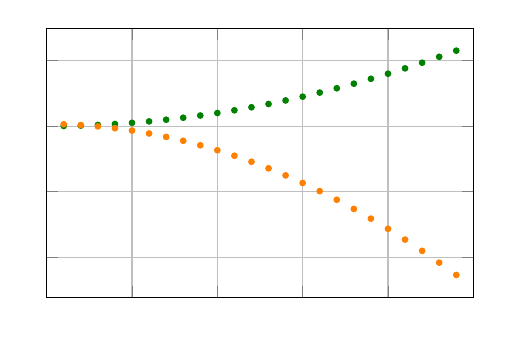
\begin{tikzpicture}
  \begin{axis}[
      xmin=0, xmax=25,
      width=7cm, height=5cm,
      grid=major,
      xticklabels={},  % Remove x-axis tick labels
      yticklabels={}
  ]
    
  \foreach \x in {1,2,...,24} {
      \addplot[dark_green, only marks, mark=*, mark size=1pt] coordinates {(\x, \x^2)};
  }
  \foreach \x in {1,2,...,24} {
    \edef\y{(16-2*\x^2)}
    \addplot[orange, only marks, mark=*, mark size=1pt] coordinates {(\x, \y)};
  }

  \end{axis}
\end{tikzpicture}
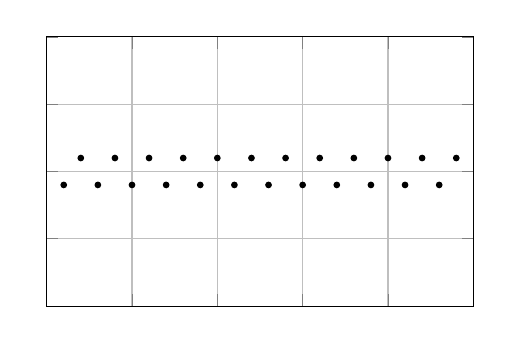
\begin{tikzpicture}
  \begin{axis}[
      xmin=0, xmax=25,
      ymin=-10, ymax=10,
      width=7cm, height=5cm,
      grid=major,
      xticklabels={},  % Remove x-axis tick labels
      yticklabels={} % Remove y-axis tick labels
  ]
    
  \foreach \x in {1,2,...,24} {
    \edef\y{((-1)^\x)}
    \addplot[only marks, mark=*, mark size=1pt] coordinates {(\x, \y)};
  }

  \end{axis}
\end{tikzpicture}


\subsection*{Limite finie}

\begin{itemize}
  \item On écrit $\displaystyle \lim_{n\to+\infty}u_n=0$ ce qui signifie que $u_n$ peut être aussi proche de $0$ que l'on veut, pourvue que $n$ soit assez grand. \\
  On le note : $\forall\epsilon>0,\exists n_0\in\mathbb{N} \quad \forall n>n_0,\left\lvert u_n\right\rvert<\epsilon $
  \item On écrit $\displaystyle \lim_{n\to+\infty}v_n=2$ ce qui signifie que $v_n$ peut être aussi proche de $2$ que l'on veut, pourvue que $n$ soit assez grand. \\
  On le note : $\forall\epsilon>0,\exists n_0\in\mathbb{N} \quad \forall n>n_0,\left\lvert v_n-2\right\rvert<\epsilon $
\end{itemize}

\subsection*{Limite infinie}

\begin{itemize}
  \item On écrit $\displaystyle \lim_{n\to+\infty}w_n=+\infty$ ce qui signifie que $w_n$ peut être aussi grand que l'on veut, pourvue que $n$ soit assez grand. \\
  On le note : $\forall A>0,\exists n_0\in\mathbb{N} \quad \forall n>n_0, w_n>A $
  \item On écrit $\displaystyle \lim_{n\to+\infty}x_n=-\infty$ ce qui signifie que $w_n$ peut être aussi petit que l'on veut, pourvue que $n$ soit assez grand. \\
  On le note : $\forall A>0,\exists n_0\in\mathbb{N} \quad \forall n>n_0, x_n<A $
\end{itemize}


\subsection*{Pas de limite}

\begin{itemize}
  \item La suite $(t_n)$ n'a pas de limite car $t_n=(-1)^n=\left\{
    \begin{array}{l}
      1 \text{ si $n$ est pair} \\
      -1 \text{ si $n$ est impair}
    \end{array}
    \right.$.
\end{itemize}

\end{document}